% Created by tikzDevice version 0.12.3.1 on 2023-02-19 18:15:29
% !TEX encoding = UTF-8 Unicode
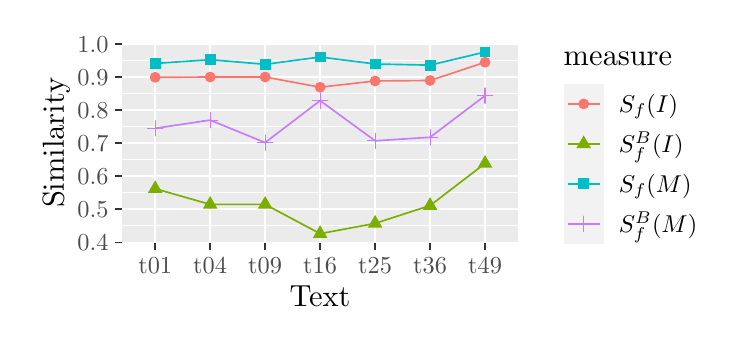
\begin{tikzpicture}[x=1pt,y=1pt]
\definecolor{fillColor}{RGB}{255,255,255}
\path[use as bounding box,fill=fillColor,fill opacity=0.00] (0,0) rectangle (252.94,108.41);
\begin{scope}
\path[clip] (  0.00,  0.00) rectangle (252.94,108.41);
\definecolor{drawColor}{RGB}{255,255,255}
\definecolor{fillColor}{RGB}{255,255,255}

\path[draw=drawColor,line width= 0.6pt,line join=round,line cap=round,fill=fillColor] (  0.00,  0.00) rectangle (252.94,108.41);
\end{scope}
\begin{scope}
\path[clip] ( 34.16, 30.69) rectangle (177.19,102.90);
\definecolor{fillColor}{gray}{0.92}

\path[fill=fillColor] ( 34.16, 30.69) rectangle (177.19,102.91);
\definecolor{drawColor}{RGB}{255,255,255}

\path[draw=drawColor,line width= 0.3pt,line join=round] ( 34.16, 36.81) --
	(177.19, 36.81);

\path[draw=drawColor,line width= 0.3pt,line join=round] ( 34.16, 48.74) --
	(177.19, 48.74);

\path[draw=drawColor,line width= 0.3pt,line join=round] ( 34.16, 60.67) --
	(177.19, 60.67);

\path[draw=drawColor,line width= 0.3pt,line join=round] ( 34.16, 72.61) --
	(177.19, 72.61);

\path[draw=drawColor,line width= 0.3pt,line join=round] ( 34.16, 84.54) --
	(177.19, 84.54);

\path[draw=drawColor,line width= 0.3pt,line join=round] ( 34.16, 96.48) --
	(177.19, 96.48);

\path[draw=drawColor,line width= 0.6pt,line join=round] ( 34.16, 30.84) --
	(177.19, 30.84);

\path[draw=drawColor,line width= 0.6pt,line join=round] ( 34.16, 42.77) --
	(177.19, 42.77);

\path[draw=drawColor,line width= 0.6pt,line join=round] ( 34.16, 54.71) --
	(177.19, 54.71);

\path[draw=drawColor,line width= 0.6pt,line join=round] ( 34.16, 66.64) --
	(177.19, 66.64);

\path[draw=drawColor,line width= 0.6pt,line join=round] ( 34.16, 78.58) --
	(177.19, 78.58);

\path[draw=drawColor,line width= 0.6pt,line join=round] ( 34.16, 90.51) --
	(177.19, 90.51);

\path[draw=drawColor,line width= 0.6pt,line join=round] ( 34.16,102.44) --
	(177.19,102.44);

\path[draw=drawColor,line width= 0.6pt,line join=round] ( 46.08, 30.69) --
	( 46.08,102.90);

\path[draw=drawColor,line width= 0.6pt,line join=round] ( 65.94, 30.69) --
	( 65.94,102.90);

\path[draw=drawColor,line width= 0.6pt,line join=round] ( 85.81, 30.69) --
	( 85.81,102.90);

\path[draw=drawColor,line width= 0.6pt,line join=round] (105.67, 30.69) --
	(105.67,102.90);

\path[draw=drawColor,line width= 0.6pt,line join=round] (125.54, 30.69) --
	(125.54,102.90);

\path[draw=drawColor,line width= 0.6pt,line join=round] (145.40, 30.69) --
	(145.40,102.90);

\path[draw=drawColor,line width= 0.6pt,line join=round] (165.27, 30.69) --
	(165.27,102.90);
\definecolor{fillColor}{RGB}{248,118,109}

\path[fill=fillColor] ( 46.08, 90.47) circle (  1.96);
\definecolor{fillColor}{RGB}{124,174,0}

\path[fill=fillColor] ( 46.08, 53.26) --
	( 48.72, 48.68) --
	( 43.43, 48.68) --
	cycle;
\definecolor{fillColor}{RGB}{0,191,196}

\path[fill=fillColor] ( 44.11, 93.52) --
	( 48.04, 93.52) --
	( 48.04, 97.44) --
	( 44.11, 97.44) --
	cycle;
\definecolor{drawColor}{RGB}{199,124,255}

\path[draw=drawColor,line width= 0.4pt,line join=round,line cap=round] ( 43.30, 72.05) -- ( 48.85, 72.05);

\path[draw=drawColor,line width= 0.4pt,line join=round,line cap=round] ( 46.08, 69.28) -- ( 46.08, 74.83);
\definecolor{fillColor}{RGB}{248,118,109}

\path[fill=fillColor] ( 65.94, 90.58) circle (  1.96);
\definecolor{fillColor}{RGB}{124,174,0}

\path[fill=fillColor] ( 65.94, 47.60) --
	( 68.58, 43.02) --
	( 63.30, 43.02) --
	cycle;
\definecolor{fillColor}{RGB}{0,191,196}

\path[fill=fillColor] ( 63.98, 94.88) --
	( 67.90, 94.88) --
	( 67.90, 98.81) --
	( 63.98, 98.81) --
	cycle;

\path[draw=drawColor,line width= 0.4pt,line join=round,line cap=round] ( 63.17, 75.00) -- ( 68.72, 75.00);

\path[draw=drawColor,line width= 0.4pt,line join=round,line cap=round] ( 65.94, 72.22) -- ( 65.94, 77.77);
\definecolor{fillColor}{RGB}{248,118,109}

\path[fill=fillColor] ( 85.81, 90.58) circle (  1.96);
\definecolor{fillColor}{RGB}{124,174,0}

\path[fill=fillColor] ( 85.81, 47.60) --
	( 88.45, 43.02) --
	( 83.16, 43.02) --
	cycle;
\definecolor{fillColor}{RGB}{0,191,196}

\path[fill=fillColor] ( 83.84, 93.20) --
	( 87.77, 93.20) --
	( 87.77, 97.12) --
	( 83.84, 97.12) --
	cycle;

\path[draw=drawColor,line width= 0.4pt,line join=round,line cap=round] ( 83.03, 66.89) -- ( 88.58, 66.89);

\path[draw=drawColor,line width= 0.4pt,line join=round,line cap=round] ( 85.81, 64.11) -- ( 85.81, 69.66);
\definecolor{fillColor}{RGB}{248,118,109}

\path[fill=fillColor] (105.67, 86.89) circle (  1.96);
\definecolor{fillColor}{RGB}{124,174,0}

\path[fill=fillColor] (105.67, 37.02) --
	(108.32, 32.44) --
	(103.03, 32.44) --
	cycle;
\definecolor{fillColor}{RGB}{0,191,196}

\path[fill=fillColor] (103.71, 95.85) --
	(107.63, 95.85) --
	(107.63, 99.77) --
	(103.71, 99.77) --
	cycle;

\path[draw=drawColor,line width= 0.4pt,line join=round,line cap=round] (102.90, 82.04) -- (108.45, 82.04);

\path[draw=drawColor,line width= 0.4pt,line join=round,line cap=round] (105.67, 79.26) -- (105.67, 84.81);
\definecolor{fillColor}{RGB}{248,118,109}

\path[fill=fillColor] (125.54, 89.15) circle (  1.96);
\definecolor{fillColor}{RGB}{124,174,0}

\path[fill=fillColor] (125.54, 40.74) --
	(128.18, 36.17) --
	(122.90, 36.17) --
	cycle;
\definecolor{fillColor}{RGB}{0,191,196}

\path[fill=fillColor] (123.58, 93.31) --
	(127.50, 93.31) --
	(127.50, 97.24) --
	(123.58, 97.24) --
	cycle;

\path[draw=drawColor,line width= 0.4pt,line join=round,line cap=round] (122.76, 67.53) -- (128.31, 67.53);

\path[draw=drawColor,line width= 0.4pt,line join=round,line cap=round] (125.54, 64.75) -- (125.54, 70.30);
\definecolor{fillColor}{RGB}{248,118,109}

\path[fill=fillColor] (145.40, 89.32) circle (  1.96);
\definecolor{fillColor}{RGB}{124,174,0}

\path[fill=fillColor] (145.40, 47.19) --
	(148.05, 42.61) --
	(142.76, 42.61) --
	cycle;
\definecolor{fillColor}{RGB}{0,191,196}

\path[fill=fillColor] (143.44, 92.91) --
	(147.37, 92.91) --
	(147.37, 96.83) --
	(143.44, 96.83) --
	cycle;

\path[draw=drawColor,line width= 0.4pt,line join=round,line cap=round] (142.63, 68.80) -- (148.18, 68.80);

\path[draw=drawColor,line width= 0.4pt,line join=round,line cap=round] (145.40, 66.02) -- (145.40, 71.57);
\definecolor{fillColor}{RGB}{248,118,109}

\path[fill=fillColor] (165.27, 95.91) circle (  1.96);
\definecolor{fillColor}{RGB}{124,174,0}

\path[fill=fillColor] (165.27, 62.40) --
	(167.91, 57.82) --
	(162.63, 57.82) --
	cycle;
\definecolor{fillColor}{RGB}{0,191,196}

\path[fill=fillColor] (163.31, 97.66) --
	(167.23, 97.66) --
	(167.23,101.58) --
	(163.31,101.58) --
	cycle;

\path[draw=drawColor,line width= 0.4pt,line join=round,line cap=round] (162.50, 83.85) -- (168.04, 83.85);

\path[draw=drawColor,line width= 0.4pt,line join=round,line cap=round] (165.27, 81.07) -- (165.27, 86.62);
\definecolor{drawColor}{RGB}{248,118,109}

\path[draw=drawColor,line width= 0.6pt,line join=round] ( 46.08, 90.47) --
	( 65.94, 90.58) --
	( 85.81, 90.58) --
	(105.67, 86.89) --
	(125.54, 89.15) --
	(145.40, 89.32) --
	(165.27, 95.91);
\definecolor{drawColor}{RGB}{124,174,0}

\path[draw=drawColor,line width= 0.6pt,line join=round] ( 46.08, 50.21) --
	( 65.94, 44.55) --
	( 85.81, 44.55) --
	(105.67, 33.97) --
	(125.54, 37.69) --
	(145.40, 44.13) --
	(165.27, 59.35);
\definecolor{drawColor}{RGB}{0,191,196}

\path[draw=drawColor,line width= 0.6pt,line join=round] ( 46.08, 95.48) --
	( 65.94, 96.84) --
	( 85.81, 95.16) --
	(105.67, 97.81) --
	(125.54, 95.28) --
	(145.40, 94.87) --
	(165.27, 99.62);
\definecolor{drawColor}{RGB}{199,124,255}

\path[draw=drawColor,line width= 0.6pt,line join=round] ( 46.08, 72.05) --
	( 65.94, 75.00) --
	( 85.81, 66.89) --
	(105.67, 82.04) --
	(125.54, 67.53) --
	(145.40, 68.80) --
	(165.27, 83.85);
\end{scope}
\begin{scope}
\path[clip] (  0.00,  0.00) rectangle (252.94,108.41);
\definecolor{drawColor}{gray}{0.30}

\node[text=drawColor,anchor=base east,inner sep=0pt, outer sep=0pt, scale=  0.88] at ( 29.21, 27.81) {0.4};

\node[text=drawColor,anchor=base east,inner sep=0pt, outer sep=0pt, scale=  0.88] at ( 29.21, 39.74) {0.5};

\node[text=drawColor,anchor=base east,inner sep=0pt, outer sep=0pt, scale=  0.88] at ( 29.21, 51.68) {0.6};

\node[text=drawColor,anchor=base east,inner sep=0pt, outer sep=0pt, scale=  0.88] at ( 29.21, 63.61) {0.7};

\node[text=drawColor,anchor=base east,inner sep=0pt, outer sep=0pt, scale=  0.88] at ( 29.21, 75.54) {0.8};

\node[text=drawColor,anchor=base east,inner sep=0pt, outer sep=0pt, scale=  0.88] at ( 29.21, 87.48) {0.9};

\node[text=drawColor,anchor=base east,inner sep=0pt, outer sep=0pt, scale=  0.88] at ( 29.21, 99.41) {1.0};
\end{scope}
\begin{scope}
\path[clip] (  0.00,  0.00) rectangle (252.94,108.41);
\definecolor{drawColor}{gray}{0.20}

\path[draw=drawColor,line width= 0.6pt,line join=round] ( 31.41, 30.84) --
	( 34.16, 30.84);

\path[draw=drawColor,line width= 0.6pt,line join=round] ( 31.41, 42.77) --
	( 34.16, 42.77);

\path[draw=drawColor,line width= 0.6pt,line join=round] ( 31.41, 54.71) --
	( 34.16, 54.71);

\path[draw=drawColor,line width= 0.6pt,line join=round] ( 31.41, 66.64) --
	( 34.16, 66.64);

\path[draw=drawColor,line width= 0.6pt,line join=round] ( 31.41, 78.58) --
	( 34.16, 78.58);

\path[draw=drawColor,line width= 0.6pt,line join=round] ( 31.41, 90.51) --
	( 34.16, 90.51);

\path[draw=drawColor,line width= 0.6pt,line join=round] ( 31.41,102.44) --
	( 34.16,102.44);
\end{scope}
\begin{scope}
\path[clip] (  0.00,  0.00) rectangle (252.94,108.41);
\definecolor{drawColor}{gray}{0.20}

\path[draw=drawColor,line width= 0.6pt,line join=round] ( 46.08, 27.94) --
	( 46.08, 30.69);

\path[draw=drawColor,line width= 0.6pt,line join=round] ( 65.94, 27.94) --
	( 65.94, 30.69);

\path[draw=drawColor,line width= 0.6pt,line join=round] ( 85.81, 27.94) --
	( 85.81, 30.69);

\path[draw=drawColor,line width= 0.6pt,line join=round] (105.67, 27.94) --
	(105.67, 30.69);

\path[draw=drawColor,line width= 0.6pt,line join=round] (125.54, 27.94) --
	(125.54, 30.69);

\path[draw=drawColor,line width= 0.6pt,line join=round] (145.40, 27.94) --
	(145.40, 30.69);

\path[draw=drawColor,line width= 0.6pt,line join=round] (165.27, 27.94) --
	(165.27, 30.69);
\end{scope}
\begin{scope}
\path[clip] (  0.00,  0.00) rectangle (252.94,108.41);
\definecolor{drawColor}{gray}{0.30}

\node[text=drawColor,anchor=base,inner sep=0pt, outer sep=0pt, scale=  0.88] at ( 46.08, 19.68) {t01};

\node[text=drawColor,anchor=base,inner sep=0pt, outer sep=0pt, scale=  0.88] at ( 65.94, 19.68) {t04};

\node[text=drawColor,anchor=base,inner sep=0pt, outer sep=0pt, scale=  0.88] at ( 85.81, 19.68) {t09};

\node[text=drawColor,anchor=base,inner sep=0pt, outer sep=0pt, scale=  0.88] at (105.67, 19.68) {t16};

\node[text=drawColor,anchor=base,inner sep=0pt, outer sep=0pt, scale=  0.88] at (125.54, 19.68) {t25};

\node[text=drawColor,anchor=base,inner sep=0pt, outer sep=0pt, scale=  0.88] at (145.40, 19.68) {t36};

\node[text=drawColor,anchor=base,inner sep=0pt, outer sep=0pt, scale=  0.88] at (165.27, 19.68) {t49};
\end{scope}
\begin{scope}
\path[clip] (  0.00,  0.00) rectangle (252.94,108.41);
\definecolor{drawColor}{RGB}{0,0,0}

\node[text=drawColor,anchor=base,inner sep=0pt, outer sep=0pt, scale=  1.10] at (105.67,  7.64) {Text};
\end{scope}
\begin{scope}
\path[clip] (  0.00,  0.00) rectangle (252.94,108.41);
\definecolor{drawColor}{RGB}{0,0,0}

\node[text=drawColor,rotate= 90.00,anchor=base,inner sep=0pt, outer sep=0pt, scale=  1.10] at ( 13.08, 66.80) {Similarity};
\end{scope}
\begin{scope}
\path[clip] (  0.00,  0.00) rectangle (252.94,108.41);
\definecolor{fillColor}{RGB}{255,255,255}

\path[fill=fillColor] (188.19, 24.78) rectangle (247.44,108.81);
\end{scope}
\begin{scope}
\path[clip] (  0.00,  0.00) rectangle (252.94,108.41);
\definecolor{drawColor}{RGB}{0,0,0}

\node[text=drawColor,anchor=base west,inner sep=0pt, outer sep=0pt, scale=  1.10] at (193.69, 94.67) {measure};
\end{scope}
\begin{scope}
\path[clip] (  0.00,  0.00) rectangle (252.94,108.41);
\definecolor{fillColor}{gray}{0.95}

\path[fill=fillColor] (193.69, 73.64) rectangle (208.14, 88.10);
\end{scope}
\begin{scope}
\path[clip] (  0.00,  0.00) rectangle (252.94,108.41);
\definecolor{fillColor}{RGB}{248,118,109}

\path[fill=fillColor] (200.92, 80.87) circle (  1.96);
\end{scope}
\begin{scope}
\path[clip] (  0.00,  0.00) rectangle (252.94,108.41);
\definecolor{drawColor}{RGB}{248,118,109}

\path[draw=drawColor,line width= 0.6pt,line join=round] (195.13, 80.87) -- (206.70, 80.87);
\end{scope}
\begin{scope}
\path[clip] (  0.00,  0.00) rectangle (252.94,108.41);
\definecolor{fillColor}{gray}{0.95}

\path[fill=fillColor] (193.69, 59.19) rectangle (208.14, 73.64);
\end{scope}
\begin{scope}
\path[clip] (  0.00,  0.00) rectangle (252.94,108.41);
\definecolor{fillColor}{RGB}{124,174,0}

\path[fill=fillColor] (200.92, 69.47) --
	(203.56, 64.89) --
	(198.27, 64.89) --
	cycle;
\end{scope}
\begin{scope}
\path[clip] (  0.00,  0.00) rectangle (252.94,108.41);
\definecolor{drawColor}{RGB}{124,174,0}

\path[draw=drawColor,line width= 0.6pt,line join=round] (195.13, 66.42) -- (206.70, 66.42);
\end{scope}
\begin{scope}
\path[clip] (  0.00,  0.00) rectangle (252.94,108.41);
\definecolor{fillColor}{gray}{0.95}

\path[fill=fillColor] (193.69, 44.73) rectangle (208.14, 59.19);
\end{scope}
\begin{scope}
\path[clip] (  0.00,  0.00) rectangle (252.94,108.41);
\definecolor{fillColor}{RGB}{0,191,196}

\path[fill=fillColor] (198.95, 50.00) --
	(202.88, 50.00) --
	(202.88, 53.92) --
	(198.95, 53.92) --
	cycle;
\end{scope}
\begin{scope}
\path[clip] (  0.00,  0.00) rectangle (252.94,108.41);
\definecolor{drawColor}{RGB}{0,191,196}

\path[draw=drawColor,line width= 0.6pt,line join=round] (195.13, 51.96) -- (206.70, 51.96);
\end{scope}
\begin{scope}
\path[clip] (  0.00,  0.00) rectangle (252.94,108.41);
\definecolor{fillColor}{gray}{0.95}

\path[fill=fillColor] (193.69, 30.28) rectangle (208.14, 44.73);
\end{scope}
\begin{scope}
\path[clip] (  0.00,  0.00) rectangle (252.94,108.41);
\definecolor{drawColor}{RGB}{199,124,255}

\path[draw=drawColor,line width= 0.4pt,line join=round,line cap=round] (198.14, 37.51) -- (203.69, 37.51);

\path[draw=drawColor,line width= 0.4pt,line join=round,line cap=round] (200.92, 34.73) -- (200.92, 40.28);
\end{scope}
\begin{scope}
\path[clip] (  0.00,  0.00) rectangle (252.94,108.41);
\definecolor{drawColor}{RGB}{199,124,255}

\path[draw=drawColor,line width= 0.6pt,line join=round] (195.13, 37.51) -- (206.70, 37.51);
\end{scope}
\begin{scope}
\path[clip] (  0.00,  0.00) rectangle (252.94,108.41);
\definecolor{drawColor}{RGB}{0,0,0}

\node[text=drawColor,anchor=base west,inner sep=0pt, outer sep=0pt, scale=  0.88] at (213.64, 77.84) {$S_f(I)$};
\end{scope}
\begin{scope}
\path[clip] (  0.00,  0.00) rectangle (252.94,108.41);
\definecolor{drawColor}{RGB}{0,0,0}

\node[text=drawColor,anchor=base west,inner sep=0pt, outer sep=0pt, scale=  0.88] at (213.64, 63.38) {$S_f^B(I)$};
\end{scope}
\begin{scope}
\path[clip] (  0.00,  0.00) rectangle (252.94,108.41);
\definecolor{drawColor}{RGB}{0,0,0}

\node[text=drawColor,anchor=base west,inner sep=0pt, outer sep=0pt, scale=  0.88] at (213.64, 48.93) {$S_f(M)$};
\end{scope}
\begin{scope}
\path[clip] (  0.00,  0.00) rectangle (252.94,108.41);
\definecolor{drawColor}{RGB}{0,0,0}

\node[text=drawColor,anchor=base west,inner sep=0pt, outer sep=0pt, scale=  0.88] at (213.64, 34.48) {$S_f^B(M)$};
\end{scope}
\end{tikzpicture}
